% 教材原图可点击，指向发布时的原图文件。
\newcommand{\effectcredit}[2]{\par{\footnotesize\color{muted}教材图 © Joey de Vries
  (\href{https://twitter.com/JoeyDeVriez}{@JoeyDeVriez})，
  \href{#1}{LearnOpenGL · #2}，
  \href{https://creativecommons.org/licenses/by/4.0/}{CC BY 4.0}。原图按比例排版。}\par}

\clearpage
\section{方向光的阴影边缘}
观察木地板上的影子。盒子的边是直的，影子边缘却出现了小台阶。阴影图记录灯光在每个像素看见的最近表面。地板上的多个点落进同一个阴影像素时，它们会一起变亮或一起变暗。右图沿同一条边多看了几个邻居，暗到亮之间便多了几级。
\begin{figure}[H]\centering
\href{https://learnopengl.com/img/advanced-lighting/shadow_mapping_zoom.png}{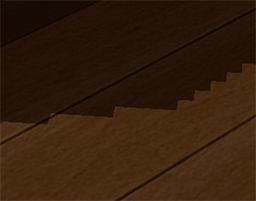
\includegraphics[height=3.4cm]{figures/effects-hard.png}}\hfill
\href{https://learnopengl.com/img/advanced-lighting/shadow_mapping_soft_shadows.png}{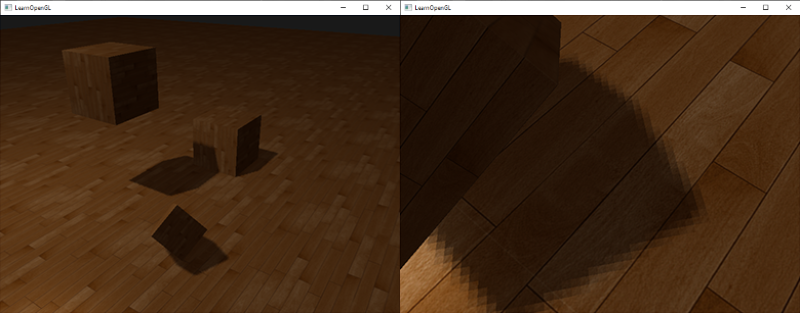
\includegraphics[height=3.4cm]{figures/effects-pcf.png}}
\caption{左图放大了单次比较的台阶。右侧原图给出多点比较后的全景和局部，局部仍能看见离散采样留下的过渡带。}
\effectcredit{https://learnopengl.com/Advanced-Lighting/Shadows/Shadow-Mapping}{Shadow Mapping，PCF}
\end{figure}

设地板上一点的灯光深度为 $z$，阴影图在邻居 $j$ 处记下的深度是 $D_j$。两者都已映射到 $[0,1]$，沿灯光方向越远数值越大。给 $z$ 减去一点余量 $b$，可以减轻地板错误遮住自己的斑点。若 $z-b\le D_j$，这一次比较就认为灯光可见。PCF（Percentage-Closer Filtering）将多次判断取平均。Redflag 在小半径分支计算
\[
 V=\frac{1}{9}\sum_{j=1}^{9}\mathbf 1[z-b\le D_j].
\]
九个位置组成 $3\times3$ 方格，横竖相邻点在阴影图上相隔一个像素。先看函数如何判定一次受光，再看外层如何累计同一种结果。
\begin{lstlisting}
return refDepth <= occ ? 1.0 : 0.0;
\end{lstlisting}
\begin{lstlisting}
sum += SampleShadow(baseUV + vec2(x, y) * texel, refDepth);
return sum / 9.0;
\end{lstlisting}
\loc{RedflagForge/assets/shaders/Renderer3D_Mesh.glsl}{SampleShadow、PCF3x3}
例如 $z-b=0.60$，九个深度中六个为 $0.70$，另外三个为 $0.55$，这盏方向光的可见比例就是 $6/9$。走到影子里面，九个位置都看到前面的盒子，这一项降到零。项目里只有第一盏方向光使用这张阴影图。场景中的其他光仍可照亮地板。

\clearpage
\section{屏幕空间环境遮蔽}
看右图 Cornell Box 里箱子贴近地板的位置。地板中央能接到上方许多方向的光，贴着箱子的地方有一侧被挡住。屏幕空间环境遮蔽（SSAO）用相机已经画出的深度估计这种差别。图中还包括方向光阴影和间接光；只凭成图的暗边无法分清各自贡献。
\begin{figure}[H]\centering
\href{https://learnopengl.com/img/advanced-lighting/ssao_hemisphere.png}{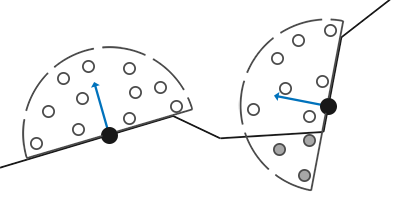
\includegraphics[width=.43\linewidth]{figures/effects-ssao.png}}\hfill
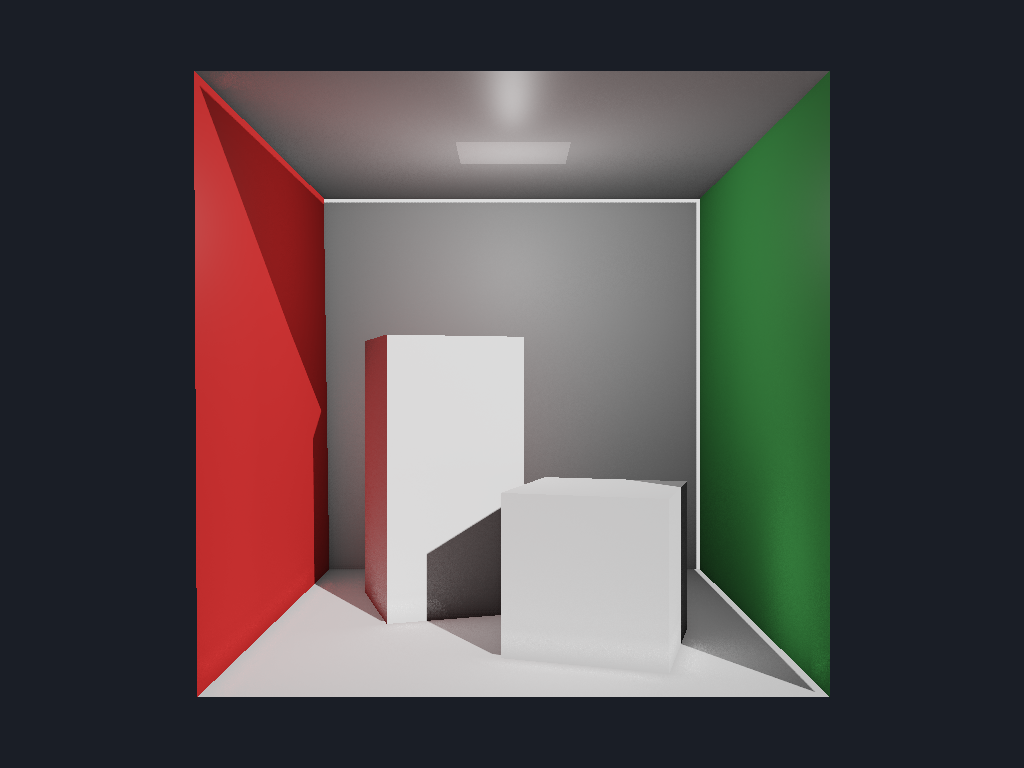
\includegraphics[height=3.8cm]{../../../output/scenes/CornellBox.png}
\caption{左图的蓝箭头指向表面外侧。让半球随箭头转动，地板上的点就只检查地板上方。右图为 Redflag 的 Cornell Box，取自 \texttt{tests/scenes/cornell.yaml} 配置的第 12 帧。}
\effectcredit{https://learnopengl.com/Advanced-Lighting/SSAO}{SSAO，Normal-oriented hemisphere}
\end{figure}

先由当前像素深度反推出观察空间位置 $p$。以表面法线 $N$ 和两个切线方向 $T,B$ 为轴，将单位半球内的样本 $s_i$ 放到测试位置 $q_i=p+r[T\,B\,N]s_i$。半径 $r$ 和 $p$ 使用相同的场景长度单位。把 $q_i$ 投回屏幕，从深度图恢复相机实际看见的表面 $z_i$。相机朝负 $Z$，例如 $-2.8$ 比 $-3.0$ 更靠近相机。若 $z_i\ge q_{i,z}+b$，就记为一次遮挡，$b$ 是同样以场景长度计的余量。
\[
 A=\left(1-\frac{1}{K}\sum_{i=1}^{K} w_i\,\mathbf 1[z_i\ge q_{i,z}+b]\right)^{s}.
\]
$w_i$ 在 $0$ 和 $1$ 之间。当前表面与采到的表面相距很远时，着色器减小它的权重，避免远墙的轮廓在近处物体边缘印出黑圈。屏幕外的样本贡献为零，分母仍是全部 $K$ 个样本。$s$ 决定遮蔽处的明暗。
\begin{lstlisting}
occlusion += (sceneZ >= samplePos.z + bias ? 1.0 : 0.0) * rangeCheck;
occlusion = 1.0 - occlusion / float(kernelSize);
float ao  = pow(clamp(occlusion, 0.0, 1.0), u_Params.z);
\end{lstlisting}
\loc{RedflagForge/assets/shaders/SSAO.glsl}{main（片元阶段，节选）}
例如四个等权样本中只有一个被挡，$s=2$，留下的环境光比例为 $(1-1/4)^2=0.5625$。单独查看 SSAO 灰度图时，这个位置应呈灰色；回到主画面，这个数只衰减环境项。移到屏幕外的物体没有深度记录，无法参加这一估算。

\clearpage
\section{环境贴图照明与粗糙度}
抛光金属能映出一扇窗的轮廓，磨粗的金属上，同一扇窗会散成一片亮斑。Redflag 把四周各方向的亮度存进一张立方体贴图。环境贴图照明（IBL）从中计算两种不同的结果，漫反射随表面朝向变化，镜面反射还随观察方向和粗糙度变化。
\begin{figure}[H]\centering
\href{https://learnopengl.com/img/pbr/ibl_hemisphere_sample_normal.png}{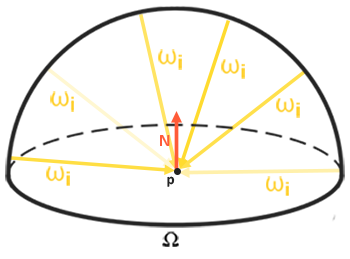
\includegraphics[height=2.7cm]{figures/effects-irradiance.png}}\hfill
\href{https://learnopengl.com/img/pbr/ibl_specular_lobe.png}{
\includegraphics[width=.64\linewidth]{figures/effects-specular.png}}
\caption{左图沿法线上方的半球汇总照明。右图从左到右越来越粗糙，能对倒影产生影响的方向也越来越多。}
\effectcredit{https://learnopengl.com/PBR/IBL/Diffuse-irradiance}{Diffuse irradiance}
{\footnotesize\color{muted}右图同作者、同许可，出自 \href{https://learnopengl.com/PBR/IBL/Specular-IBL}{Specular IBL}。}
\end{figure}

设环境从方向 $\omega$ 送来的线性 RGB 为 $L(\omega)$，它与法线 $N$ 的夹角为 $\theta$。正对表面的光比擦过表面的光更有效，因此用 $\cos\theta$ 加权。漫反射还要除以 $\pi$，项目在预计算时已经做了这一步。着色时沿 $N$ 取一次贴图，再乘材质颜色 $\rho$ 就得到 $\rho D(N)$：
\[
D(N)=\frac{1}{\pi}\int_{\Omega^+(N)}L(\omega)\cos\theta\,\mathrm d\omega,\qquad
\mathrm d\omega=\sin\theta\,\mathrm d\theta\,\mathrm d\phi .
\]
按经纬角等步长取样时，每格立体角带有 $\sin\theta$。两个角度的范围乘积是 $\pi^2$，除以漫反射的 $\pi$ 后，程序给样本平均值乘 $\pi$。
\begin{lstlisting}
irr += texture(u_EnvMap, w).rgb * cos(theta) * sin(theta);
irr = PI * irr / count;
\end{lstlisting}
\loc{Redflag/src/Redflag/Renderer/IBLPrecompute.cpp}{s\_IrradianceFS（漫反射预计算）}
镜面项沿视线的反射方向查另一张预先模糊的环境图。粗糙度从 $0$ 变为 $1$，读取的层级从 $0$ 变为 $4$。一张二维表保存了视线角度和粗糙度对应的两个系数 $a,b$，用来调整镜面反射颜色 $k_S$：
\[
 L_{\rm env}=A\,[k_D\,\rho D(N)+L_{\rm filtered}(R,4r)(k_S a+b)].
\]
这里 $r$ 表示粗糙度，$A$ 合并了材质和屏幕空间的遮蔽。项目把它同时乘在环境漫反射和镜面反射上。
\begin{lstlisting}
vec3 specularIBL = prefilteredColor * (kS * brdf.x + brdf.y);
ambient = (kD * diffuseIBL + specularIBL) * ao;
\end{lstlisting}
\loc{RedflagForge/assets/shaders/Renderer3D_Mesh.glsl}{main（片元阶段，节选）}
如果六面环境图都是 $(2,1,0.5)$，任何朝向应得到同样的 $D$，模糊一块纯色也应保留该颜色。\path{tests/run_ibl_tests.cmd} 正是这样检查立方体六面。上一页的 Cornell 截图关闭了 IBL；墙面反弹到地板上的红光来自下一节的反射阴影图。

\newpage
\section{RSM 的反射通量与面积}
方向光照亮红墙后，红墙会向地面反射一部分光。RSM（反射阴影图）先保存光源能看到的表面，再把这些表面当作小光源收集贡献。这条路径只有一次间接漫反射，没有继续计算地面把光反射给第三个表面。

\begin{figure}[H]\centering
\begin{tikzpicture}[scale=.95]
\fill[pale] (1,0) rectangle (1.2,3.3);
\fill[pale] (1,0) rectangle (8.3,-.2);
\draw[thick,blue] (1,3.3)--(1,0)--(8.3,0);
\fill[red!65!black] (1,2.3) circle(2.5pt) node[left=3pt] {$y$};
\fill[ink] (5.7,0) circle(2.5pt) node[below=3pt] {$x$};
\draw[flow] (3.1,3.3)--node[label,above] {方向光}(1.05,2.33);
\draw[flow,draw=red!65!black] (1.08,2.26)--node[label,above] {$\omega=(x-y)/r$}(5.64,.04);
\draw[flow] (1,2.3)--(2,2.3) node[right] {$n_y$};
\draw[flow] (5.7,0)--(5.7,1) node[above] {$n_x$};
\draw[flow] (5.8,.1)--node[label,right] {朝相机反射}(7.2,1.7);
\node[font=\small] at (2.7,.45) {红墙};
\node[font=\small] at (7.5,.35) {地面};
\end{tikzpicture}
\caption{本文绘制的光路示意。$y$ 是发送点，$x$ 是接收点，两端的位置和法线都使用世界空间。}
\end{figure}

\subsection{从表面面积换到光源投影面积}
设方向光正交范围宽 $w=2h$，覆盖面积 $A=w^2$。光源纹理有 $W\times H$ 个像素，每个像素对应的投影面积为 $\Delta A_\perp=A/(WH)$。这些面积使用场景长度单位的平方，不是屏幕像素面积。

令 $q$ 为方向光垂直截面的辐照度，$c_l=\max(n_y\cdot l,0)$，$l$ 从表面指向光源。发送面的实际面积 $\mathrm dA_y$ 投影后变为 $\mathrm dA_\perp=c_l\,\mathrm dA_y$。用 $C_y$ 表示线性底色，当前采用漫反射率 $\rho_y=(1-m_y)C_y$，于是
\[
 \mathrm d\Phi_y=\rho_y\,q\,c_l\,\mathrm dA_y
                =\rho_y\,q\,\mathrm dA_\perp.
\]
斜面单位实际面积收到的光较少，但一个光源像素覆盖的实际面积更大，两项抵消。因此按投影面积记录反射通量时，不再乘一次 $c_l$。背光面仍需排除。

Redflag 的 RGBA16F 附件存 $D_y=\rho_y q$，即\textbf{每单位光源投影面积的反射通量}。每纹素的通量应为 $\Phi_y=D_y\Delta A_\perp$。存密度后，可以把面积留到收集阶段乘入，避免先存很小的纹素通量、再乘回纹素数量。灯光数值未做物理标定，$q$ 在项目中仍是颜色乘强度。

\note{原算法依据：Dachsbacher、Stamminger，\source{https://users.soe.ucsc.edu/~pang/160/s13/proposal/mijallen/proposal/media/p203-dachsbacher.pdf}{Reflective Shadow Maps，I3D 2005，§3.1--3.2，印刷页 204}。原文以离散纹素通量组织计算。本文的密度定义和面积整理针对 Redflag，不把二者记成同一个量。}

\newpage
\subsection{几何因子与两个 Lambert 系数}
距离为 $r=\lVert x-y\rVert$，方向 $\omega=(x-y)/r$。发送面朝接收点的余弦为 $c_y=\max(n_y\cdot\omega,0)$，接收面朝发送点的余弦为 $c_x=\max(n_x\cdot(-\omega),0)$。不考虑两点之间遮挡时，几何因子为
\[
 G(x,y)=\frac{c_y c_x}{r^2}.
\]
原论文式（1）分子用的是未经单位化的位移向量，因而写成距离四次方。两个点积各带一个 $r$，化简后仍是 $c_yc_x/r^2$。项目先得到单位方向 \code{dirN}，原来的距离平方衰减并没有少除一次距离。

Lambert 漫反射的 BRDF 是 $\rho/\pi$。发送面出射辐亮度为 $L_y=\rho_y q c_l/\pi$，再经接收面反射，有
\begin{align*}
 L_x&=\frac{\rho_x}{\pi}\int L_y\,G(x,y)\,\mathrm dA_y\\
    &=\frac{\rho_x}{\pi^2}\int D_y\,G(x,y)\,\mathrm dA_\perp.
\end{align*}
这里暂取两点可见性为 1，这是当前 RSM 的主要近似。原论文式（1）没有显式列出这里的两个 Lambert 系数，对照时需单独核算通量定义与归一化。本节保留发送、接收两端各一个 $1/\pi$，不能再从别处重复乘除。

\subsection{圆盘采样与归一化}
接收点投到光源纹理后，在 UV 半径 $R$ 的圆盘内取 $N$ 个样本。当前正交范围是正方形，这个圆盘的世界投影面积为 $A_D=A\pi R^2=\pi(wR)^2$。均匀面积采样的积分估计为
\[
 \widehat L_x=\rho_x\,\underbrace{\frac{A\pi R^2}{\pi^2N}
      \sum_{i=0}^{N-1} D_i G_i}_{\text{RSM 输出，等于接收辐照度除以 }\pi}.
\]
主绘制再乘接收材质的 $\rho_x=(1-m_x)C_x$，$C_x$ 是接收面线性底色。$\text{Intensity}$ 是额外外观倍率，默认 1。UV 越界或没有表面的样本按零贡献处理，仍除请求的 $N$，不能通过只除有效样本数把边界重新照亮。

Vogel 圆盘使用 $r_i=\sqrt{(i+0.5)/N}$。原实现分母固定为 128，只取前 16 个时，覆盖半径约为原来的 $\sqrt{16/128}\approx0.354$。现在按实际 $N$ 生成，降低质量不会同时大幅缩小覆盖范围。等面积分布使用相同权重，不能照搬原论文另一种采样分布的径向权重。

\note{Lambert 系数依据：\source{https://pbr-book.org/4ed/Reflection_Models/Diffuse_Reflection}{PBRT 第四版 §9.2：Diffuse Reflection}。RSM 几何因子对照原论文式（1）、印刷页 204。本页圆盘估计式由上述密度与等面积采样推得。}

\newpage
\subsection{源码修改与数值例}
\textbf{修改前。}以下两句取自提交 \code{1a168c3}，分别位于 RSMDepth 的片元 \code{main} 与 RSMIndirect 的 \code{ComputeRSMIndirect}。前一句多乘入射余弦，后一句只求平均，缺少圆盘投影面积与本节约定的 Lambert 系数。
\begin{lstlisting}[title={旧实现，分属两个函数}]
o_Flux     = vec4(albedo * lightColor * NdL, 1.0);
return indirect * (intensity / float(numSamples));
\end{lstlisting}

\textbf{修改后。}发送端先读取标量或贴图中的金属度。正面输出通量密度，背面输出零。下面摘出实际表达式，省略金属贴图读取和朝向判断。
\begin{lstlisting}
vec3 diffuse = baseColor.rgb * (1.0 - metallic);
fluxDensity = diffuse * u_DirLights[0].Color.rgb * u_DirLights[0].Color.w;
o_Flux     = vec4(fluxDensity, 1.0);
\end{lstlisting}
\loc{RedflagForge/assets/shaders/RSMDepth.glsl}{main（片元阶段）}

收集阶段把平均值乘圆盘面积，并计入两个 Lambert 系数。主绘制使用相同的漫反射材质约定，纯金属不再贡献这一项。
\begin{lstlisting}
float radius = sampleRadius * lightWidth;
return indirect * (intensity * radius * radius / (PI * float(numSamples)));
\end{lstlisting}
\loc{RedflagForge/assets/shaders/RSMIndirect.glsl}{ComputeRSMIndirect}
\begin{lstlisting}
Lo += texture(u_RSMResolved, screenUV).rgb * albedo * (1.0 - metallic);
\end{lstlisting}
\loc{RedflagForge/assets/shaders/Renderer3D_Mesh.glsl}{main（片元阶段）}

\textbf{数值例。}只看单通道，令 $w=10$、$R=0.2$、$q=2$、$\rho_y=0.5$，则 $D_y=1$。假设整盘的 $G=0.25$，RSM 输出为
\[
 \frac{(10\times0.2)^2}{\pi}\,(1\times0.25)=\frac1\pi\approx0.31831.
\]
接收面 $\rho_x=0.8$ 时，输出约 $0.25465$。若几何及光源覆盖一起放大两倍，面积放大四倍，$G$ 缩为四分之一，亮度保持不变。这个人为常量算例检查系数和尺度，不代表实际场景中各点的 $G$ 相同。

\newpage
\subsection{近距离处理与验证边界}
光源像素代表一小块表面，不能在两点靠近时仍把它当成无面积的无限亮点。当前用一个光源纹素的宽度 $\delta=w/W$ 限制分母：
\[
 G_{\rm used}=\frac{c_yc_x}{\max(r^2,\delta^2)},\qquad r>0.
\]
两点重合时方向无定义，代码直接跳过。这个限制替换了固定场景单位下的 \code{DIST\_BIAS=0.05} 和几何因子上限 4。新限制随光源覆盖尺度变化，但仍不是对有限面积光源的精确积分。改变 RSM 分辨率会改变这段近距离近似，不能声称已经完全分辨率无关。

\subsection{算法仍省略的内容}
两个表面之间没有再做遮挡查询。红墙可能隔着一层挡板照亮地面，这种漏光在原 RSM 中就存在，修正面积和强度不能消除。有限采样半径也会舍弃远处反射面，因此半径改变的是积分范围，不只改变噪点多少。

这里只收集第一盏方向光直接照到的表面。没有继续传播多次反射，也没有处理间接镜面反射。$(1-m)c$ 是当前漫反射近似，没有把直接光的完整 Fresnel 方向分配搬进收集积分。法线贴图细节也未参与发送面法线。不能把纯金属不再收到漫反射，解释成已经实现了金属的间接镜面光。

历史混合只根据相机重投影，没有前帧深度拒绝和物体运动信息。它能平滑一部分噪点，不能修复遮挡缺失或错误能量。调试公式时应先检查当前帧间接光，再检查多帧历史。

\subsection{复算与实测记录}
随文 \path{verify.py} 检查余弦写法等价、投影面积抵消、圆盘系数以及统一缩放后的结果。它是 CPU 数学复算，不替代实际 Shader 测试。

\subsection{从公式回到像素}

先取一个方便手算的例子，只看红色通道。设投影边长 $w=10$，纹理坐标半径 $R=0.2$，墙面收到的光 $q=2$，反射率 $\rho_y=0.5$，于是光源图上存的是 $D_y=1$。假设整个圆盘上朝向和距离合起来给出 $G=0.25$。代入上页公式，白色表面的结果为 $(10\times0.2)^2\times 0.25/\pi\approx0.31831$。地面反射率为 $0.8$ 时，朝相机的结果约为 $0.25465$。若墙、地面和灯的覆盖范围一起放大两倍，圆盘面积变成四倍，$G$ 则降为四分之一，两者相抵。随文的 \path{verify.py} 用这组数复核系数、投影面积和尺度。

显卡测试使用另一组容易判断的输入。\path{tests/Renderer3DTests.cpp} 让 RSM 纹理处处返回 $(1,0.25,0)$，两面正对、相隔 1，投影边长为 4，纹理坐标半径为 0.2。此时红色通道应为 $0.8^2/\pi\approx0.20372$，OpenGL 实际读回与公式相差不到 0.001。只把距离改为 2，亮度降为原来的四分之一。反过来改变投影宽度和纹理坐标半径、让两者乘积保持相同，结果也相同。

最后回看 Cornell 的地面 A。最早的参考图把方向光照向绿墙，光源图里红墙的反射通量为零，调高间接光强度也不会让这堵墙染红地板。把灯转向红墙，再固定同一相机、灯光和强度 5 做算法前后对照，A 点的间接增量从 $(0.07715,0.03076,0.03076)$ 变成 $(0.48218,0.13550,0.13550)$。本节开头的展示图把强度调回 1，A 点的红色增量为 0.09644。先查灯有没有照到墙，再在固定强度下比较同一块地面，就能分清灯光方向和代码改动各自带来的变化。原始读数见 \path{output/scenes/rsm/measurements.csv}。

\subsection{仍会出现的误差}

收集阶段默认墙上的样本能照到地面。若在两点之间放一块挡板，程序仍可能把红光算过去。圆盘之外的反射面则完全收不到。靠近墙脚时，把最小距离从旧版固定的 \code{DIST\_BIAS=0.05} 与几何因子上限 4，改为随纹素宽度取值，能抑制很近的亮点。光源分辨率改变后，这一近似仍会跟着变。\source{https://doi.org/10.1145/1053427.1053460}{RSM 原论文第 3.3 节讨论了遮挡近似}

目前只有第一盏方向光参与这一次间接漫反射。墙面用几何表面的插值法线，材质的法线贴图没有进入这一步。这次计算只考虑漫反射，所以纯金属既不把漫反射光送到地面，也不接收这样的光，金属的镜面反射、多次反弹和材质随角度变化的完整 Fresnel 反射都在这次估算之外。两个独立绘制测试分别检查了受光面正照与斜照、背光面与金属，以及给金属接收面加减红色输入后的结果。

相机移动时，程序把当前点投回上一帧来平滑噪点。已有的 61 项场景检查包含 16、32、128 个圆盘样本以及切换投影、光源、场景和 RSM 设置后的历史重置。普通相机移动保留历史，上一帧裁剪范围以外的点会被拒绝。同一像素上一帧是否被其他物体挡住、物体自身移动到了哪里，仍缺少对应的深度和运动数据。测试代码见 \path{tests/DepthPrepassTests.cpp} 与 \path{tests/SceneRenderTests.cpp}，运行记录见 \path{output/validation/rsm-regression.txt}。


\note{算法边界依据：原论文 §3.3 的间接光遮挡假设，以及 §7 对非漫反射扩展的讨论。实际排错过程见《Redflag 排错记录》，经典场景的图片和采集条件另见《经典场景实测》。本文不借用旧 Mask 截帧证明新的 RSM 能量计算。}


\clearpage
\section{Bloom 与亮部扩散}
图中左上的白灯亮度很高，紧挨着的木板却不会自动出现光晕。一个像素无论多亮，显示器仍只把它画在原来的位置。Bloom 先提取亮部，再把其中一部分颜色散到邻近像素，灯周围才逐渐亮起来。
\begin{figure}[H]\centering
\href{https://learnopengl.com/img/advanced-lighting/bloom_steps.png}{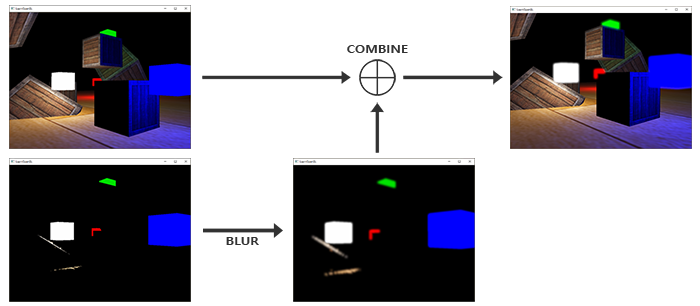
\includegraphics[width=.82\linewidth]{figures/effects-bloom.png}}
\caption{沿下方一行读图。亮部从原图中分离，模糊后再加回上方场景。白灯和蓝色亮块的轮廓仍在，周围多出一圈渐淡的颜色。}
\effectcredit{https://learnopengl.com/Advanced-Lighting/Bloom}{Bloom}
\end{figure}

Redflag 在色调映射之前提取亮部，此时线性 RGB 可以大于 $1$。它先算亮度 $Y=0.2126R+0.7152G+0.0722B$。阈值 $t$ 与 $Y$ 使用同一亮度尺度。在远高于阈值的区域，取出超过阈值的部分 $Y-t$；在阈值附近，代码用二次曲线接上，灯光慢慢变亮时光晕就不会突然跳出来。令 $\varepsilon=10^{-4}$，把亮度换成颜色保留比例的过程为
\[
\begin{aligned}
k&=\max(t/2,\varepsilon),\qquad h=\operatorname{clamp}(Y-t+k,0,2k),\\
g&=\frac{\max\!\bigl(Y-t,\,h^2/(4k+\varepsilon),\,0\bigr)}
             {\max(Y,\varepsilon)},\qquad C_{\rm bright}=\frac{gC}{1+gC}.
\end{aligned}
\]
最后的除法逐颜色分量计算。以白灯 $C=(2,2,2)$、$t=1$ 为例，$Y=2$，超过阈值的部分为 $1$，$g=1/2$，提取出的颜色为 $(0.5,0.5,0.5)$。原场景里灯的颜色仍是 $(2,2,2)$。
\begin{lstlisting}
float contribution = max(hard, soft) / max(lum, 0.0001);
vec3 bloom = c * contribution;
bloom = bloom / (vec3(1.0) + bloom);
\end{lstlisting}
\loc{RedflagForge/assets/shaders/Bloom_Brightness.glsl}{main（片元阶段，节选）}
接下来，\code{PostProcess::RenderBloom} 将亮部图逐层缩小，再从最小图向大图叠加。放大时，一个像素取周围 12 处颜色的平均值，再乘 $0.35$ 加到上一层。越小的图上，一步采样对应原图上越远的距离。这样既保住了灯边的一圈细光，又能形成宽一些的外沿。教材图演示的是提取、模糊、相加的次序；Redflag 的采样写在 \path{Bloom_Upsample.glsl}。

\clearpage
\subsection{色调映射与显示亮度}
再回到上一页右上角的图。白灯的中心即使有几倍于木板的亮度，普通显示图像的每个通道仍只能写 $0$ 到 $1$。若直接截断，高于 $1$ 的亮部都会变成同一种白。色调映射让高亮变化压进一个窄区间，稍暗的过渡仍然可见。

设场景颜色为 $C$，模糊后的亮部为 $B$，光晕强度为 $s$，曝光倍率为 $e$。项目限制加回场景的光晕每通道最多为 $1$。对有限且处在正常工作范围内的 HDR 值，先算 $x=e[C+\operatorname{clamp}(sB,0,1)]$，再逐通道代入下面的曲线。极端输入在着色器中另外限制到 $[0,64]$ 后才乘曝光。$T$ 是 Krzysztof Narkowicz 给出的 ACES 近似曲线，最后的幂运算负责将它写入当前普通 RGBA8 显示纹理：
\[
 T(x)=\operatorname{clamp}\!\left(\frac{x(2.51x+0.03)}
            {x(2.43x+0.59)+0.14},\,0,1\right),\qquad C_{\rm display}=T(x)^{1/2.2}.
\]
\begin{figure}[H]\centering
\begin{tikzpicture}[x=2.2cm,y=2.8cm,font=\footnotesize]
\draw[->,draw=muted] (0,0)--(4.2,0) node[right]{曝光后 $x$};
\draw[->,draw=muted] (0,0)--(0,1.13) node[above]{输出};
\foreach \v in {1,2,3,4}{\draw[muted] (\v,.02)--(\v,-.02) node[below]{\v};}
\foreach \v in {0,0.5,1}{\draw[muted] (.025,\v)--(-.025,\v) node[left]{\v};}
\draw[dotted,muted] (0,1)--(4.1,1);
\draw[blue,thick,domain=0:4,samples=81] plot (\x,{(\x*(2.51*\x+.03))/(\x*(2.43*\x+.59)+.14)});
\draw[ink,dashed,thick,domain=0:4,samples=81] plot (\x,{((\x*(2.51*\x+.03))/(\x*(2.43*\x+.59)+.14))^(1/2.2)});
\draw[muted,dotted] (2,0)--(2,.96);
\fill[blue] (2,.91486) circle (1.6pt);
\fill[ink] (2,.96036) circle (1.6pt);
\node[anchor=west,text=blue] at (2.35,.61) {实线：色调映射 $T(x)$};
\node[anchor=west] at (2.35,.43) {虚线：写入显示图的值};
\end{tikzpicture}
\caption{按项目着色器绘制的单通道曲线。高亮处曲线变平，$x=2$ 处的两个点对应下文取样。}
\end{figure}
\begin{lstlisting}
combined *= u_Exposure;
vec3 tonemapped = ACESTonemap(combined /* 已乘曝光的线性 RGB */);
vec3 gammaCorrected = pow(tonemapped, vec3(1.0 / 2.2));
\end{lstlisting}
\loc{RedflagForge/assets/shaders/PostProcess_Composite.glsl}{main、ACESTonemap}
遮住光晕或将其强度设为零，取单个输入通道 $C=2$、曝光 $e=1$。此时 $T(2)\approx0.91486$，最终显示值约 $0.96036$，换算为 8 位约为 $245$。所有计算都集中在同一像素，没有改变旁边木板的颜色。把倍率设为 $0$ 会得到黑色，这也是检查曝光是否真的传给这一次合成的简便办法。

做后端对照时应当先选定取样位置。同一亮点在场景 HDR 图上可以读到 $2$，在最终显示图上却只有约 $245/255$。若改用自动执行 sRGB 编码的目标，同时保留最后的 $1/2.2$ 次幂，会再提亮一次。当前 \path{tests/run_render_tests.cmd} 的后处理用例和实际合成着色器可以用来核对曝光、Bloom 开关与资源绑定。
\note{曲线系数与适用范围见 \source{https://knarkowicz.wordpress.com/2016/01/06/aces-filmic-tone-mapping-curve/}{Krzysztof Narkowicz，ACES Filmic Tone Mapping Curve}。这里的 $245$ 是由项目公式得到的数值例。}
